\documentclass[1p]{elsarticle_modified}
%\bibliographystyle{elsarticle-num}

%\usepackage[colorlinks]{hyperref}
%\usepackage{abbrmath_seonhwa} %\Abb, \Ascr, \Acal ,\Abf, \Afrak
\usepackage{amsfonts}
\usepackage{amssymb}
\usepackage{amsmath}
\usepackage{amsthm}
\usepackage{scalefnt}
\usepackage{amsbsy}
\usepackage{kotex}
\usepackage{caption}
\usepackage{subfig}
\usepackage{color}
\usepackage{graphicx}
\usepackage{xcolor} %% white, black, red, green, blue, cyan, magenta, yellow
\usepackage{float}
\usepackage{setspace}
\usepackage{hyperref}

\usepackage{tikz}
\usetikzlibrary{arrows}

\usepackage{multirow}
\usepackage{array} % fixed length table
\usepackage{hhline}

%%%%%%%%%%%%%%%%%%%%%
\makeatletter
\renewcommand*\env@matrix[1][\arraystretch]{%
	\edef\arraystretch{#1}%
	\hskip -\arraycolsep
	\let\@ifnextchar\new@ifnextchar
	\array{*\c@MaxMatrixCols c}}
\makeatother %https://tex.stackexchange.com/questions/14071/how-can-i-increase-the-line-spacing-in-a-matrix
%%%%%%%%%%%%%%%

\usepackage[normalem]{ulem}

\newcommand{\msout}[1]{\ifmmode\text{\sout{\ensuremath{#1}}}\else\sout{#1}\fi}
%SOURCE: \msout is \stkout macro in https://tex.stackexchange.com/questions/20609/strikeout-in-math-mode

\newcommand{\cancel}[1]{
	\ifmmode
	{\color{red}\msout{#1}}
	\else
	{\color{red}\sout{#1}}
	\fi
}

\newcommand{\add}[1]{
	{\color{blue}\uwave{#1}}
}

\newcommand{\replace}[2]{
	\ifmmode
	{\color{red}\msout{#1}}{\color{blue}\uwave{#2}}
	\else
	{\color{red}\sout{#1}}{\color{blue}\uwave{#2}}
	\fi
}

\newcommand{\Sol}{\mathcal{S}} %segment
\newcommand{\D}{D} %diagram
\newcommand{\A}{\mathcal{A}} %arc


%%%%%%%%%%%%%%%%%%%%%%%%%%%%%5 test

\def\sl{\operatorname{\textup{SL}}(2,\Cbb)}
\def\psl{\operatorname{\textup{PSL}}(2,\Cbb)}
\def\quan{\mkern 1mu \triangleright \mkern 1mu}

\theoremstyle{definition}
\newtheorem{thm}{Theorem}[section]
\newtheorem{prop}[thm]{Proposition}
\newtheorem{lem}[thm]{Lemma}
\newtheorem{ques}[thm]{Question}
\newtheorem{cor}[thm]{Corollary}
\newtheorem{defn}[thm]{Definition}
\newtheorem{exam}[thm]{Example}
\newtheorem{rmk}[thm]{Remark}
\newtheorem{alg}[thm]{Algorithm}

\newcommand{\I}{\sqrt{-1}}
\begin{document}

%\begin{frontmatter}
%
%\title{Boundary parabolic representations of knots up to 8 crossings}
%
%%% Group authors per affiliation:
%\author{Yunhi Cho} 
%\address{Department of Mathematics, University of Seoul, Seoul, Korea}
%\ead{yhcho@uos.ac.kr}
%
%
%\author{Seonhwa Kim} %\fnref{s_kim}}
%\address{Center for Geometry and Physics, Institute for Basic Science, Pohang, 37673, Korea}
%\ead{ryeona17@ibs.re.kr}
%
%\author{Hyuk Kim}
%\address{Department of Mathematical Sciences, Seoul National University, Seoul 08826, Korea}
%\ead{hyukkim@snu.ac.kr}
%
%\author{Seokbeom Yoon}
%\address{Department of Mathematical Sciences, Seoul National University, Seoul, 08826,  Korea}
%\ead{sbyoon15@snu.ac.kr}
%
%\begin{abstract}
%We find all boundary parabolic representation of knots up to 8 crossings.
%
%\end{abstract}
%\begin{keyword}
%    \MSC[2010] 57M25 
%\end{keyword}
%
%\end{frontmatter}

%\linenumbers
%\tableofcontents
%
\newcommand\colored[1]{\textcolor{white}{\rule[-0.35ex]{0.8em}{1.4ex}}\kern-0.8em\color{red} #1}%
%\newcommand\colored[1]{\textcolor{white}{ #1}\kern-2.17ex	\textcolor{white}{ #1}\kern-1.81ex	\textcolor{white}{ #1}\kern-2.15ex\color{red}#1	}

{\Large $\underline{12a_{0625}~(K12a_{0625})}$}

\setlength{\tabcolsep}{10pt}
\renewcommand{\arraystretch}{1.6}
\vspace{1cm}\begin{tabular}{m{100pt}>{\centering\arraybackslash}m{274pt}}
\multirow{5}{120pt}{
	\centering
	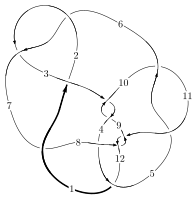
\includegraphics[width=112pt]{../../../GIT/diagram.site/Diagrams/png/1426_12a_0625.png}\\
\ \ \ A knot diagram\footnotemark}&
\allowdisplaybreaks
\textbf{Linearized knot diagam} \\
\cline{2-2}
 &
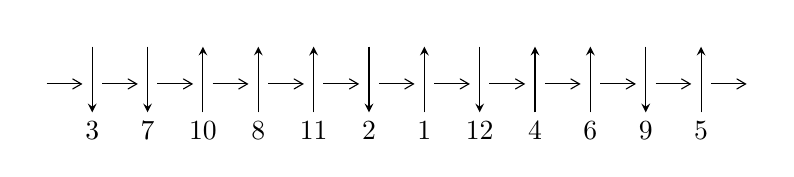
\begin{tikzpicture}[x=20pt, y=17pt]
	% nodes
	\node (C0) at (0, 0) {};
	\node (C1) at (1, 0) {};
	\node (C1U) at (1, +1) {};
	\node (C1D) at (1, -1) {3};

	\node (C2) at (2, 0) {};
	\node (C2U) at (2, +1) {};
	\node (C2D) at (2, -1) {7};

	\node (C3) at (3, 0) {};
	\node (C3U) at (3, +1) {};
	\node (C3D) at (3, -1) {10};

	\node (C4) at (4, 0) {};
	\node (C4U) at (4, +1) {};
	\node (C4D) at (4, -1) {8};

	\node (C5) at (5, 0) {};
	\node (C5U) at (5, +1) {};
	\node (C5D) at (5, -1) {11};

	\node (C6) at (6, 0) {};
	\node (C6U) at (6, +1) {};
	\node (C6D) at (6, -1) {2};

	\node (C7) at (7, 0) {};
	\node (C7U) at (7, +1) {};
	\node (C7D) at (7, -1) {1};

	\node (C8) at (8, 0) {};
	\node (C8U) at (8, +1) {};
	\node (C8D) at (8, -1) {12};

	\node (C9) at (9, 0) {};
	\node (C9U) at (9, +1) {};
	\node (C9D) at (9, -1) {4};

	\node (C10) at (10, 0) {};
	\node (C10U) at (10, +1) {};
	\node (C10D) at (10, -1) {6};

	\node (C11) at (11, 0) {};
	\node (C11U) at (11, +1) {};
	\node (C11D) at (11, -1) {9};

	\node (C12) at (12, 0) {};
	\node (C12U) at (12, +1) {};
	\node (C12D) at (12, -1) {5};
	\node (C13) at (13, 0) {};

	% arrows
	\draw[->,>={angle 60}]
	(C0) edge (C1) (C1) edge (C2) (C2) edge (C3) (C3) edge (C4) (C4) edge (C5) (C5) edge (C6) (C6) edge (C7) (C7) edge (C8) (C8) edge (C9) (C9) edge (C10) (C10) edge (C11) (C11) edge (C12) (C12) edge (C13) ;	\draw[->,>=stealth]
	(C1U) edge (C1D) (C2U) edge (C2D) (C3D) edge (C3U) (C4D) edge (C4U) (C5D) edge (C5U) (C6U) edge (C6D) (C7D) edge (C7U) (C8U) edge (C8D) (C9D) edge (C9U) (C10D) edge (C10U) (C11U) edge (C11D) (C12D) edge (C12U) ;
	\end{tikzpicture} \\
\hhline{~~} \\& 
\textbf{Solving Sequence} \\ \cline{2-2} 
 &
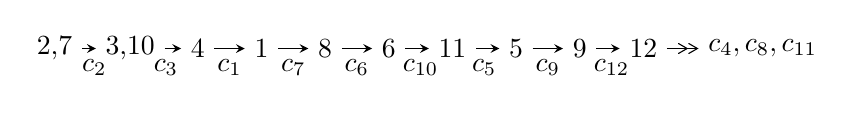
\begin{tikzpicture}[x=23pt, y=7pt]
	% node
	\node (A0) at (-1/8, 0) {2,7};
	\node (A1) at (17/16, 0) {3,10};
	\node (A2) at (17/8, 0) {4};
	\node (A3) at (25/8, 0) {1};
	\node (A4) at (33/8, 0) {8};
	\node (A5) at (41/8, 0) {6};
	\node (A6) at (49/8, 0) {11};
	\node (A7) at (57/8, 0) {5};
	\node (A8) at (65/8, 0) {9};
	\node (A9) at (73/8, 0) {12};
	\node (C1) at (1/2, -1) {$c_{2}$};
	\node (C2) at (13/8, -1) {$c_{3}$};
	\node (C3) at (21/8, -1) {$c_{1}$};
	\node (C4) at (29/8, -1) {$c_{7}$};
	\node (C5) at (37/8, -1) {$c_{6}$};
	\node (C6) at (45/8, -1) {$c_{10}$};
	\node (C7) at (53/8, -1) {$c_{5}$};
	\node (C8) at (61/8, -1) {$c_{9}$};
	\node (C9) at (69/8, -1) {$c_{12}$};
	\node (A10) at (11, 0) {$c_{4},c_{8},c_{11}$};

	% edge
	\draw[->,>=stealth]	
	(A0) edge (A1) (A1) edge (A2) (A2) edge (A3) (A3) edge (A4) (A4) edge (A5) (A5) edge (A6) (A6) edge (A7) (A7) edge (A8) (A8) edge (A9) ;
	\draw[->>,>={angle 60}]	
	(A9) edge (A10);
\end{tikzpicture} \\ 

\end{tabular} \\

\footnotetext{
The image of knot diagram is generated by the software ``\textbf{Draw programme}" developed by Andrew Bartholomew(\url{http://www.layer8.co.uk/maths/draw/index.htm\#Running-draw}), where we modified some parts for our purpose(\url{https://github.com/CATsTAILs/LinksPainter}).
}\phantom \\ \newline 
\centering \textbf{Ideals for irreducible components\footnotemark of $X_{\text{par}}$} 
 
\begin{align*}
I^u_{1}&=\langle 
-1457 u^{41}-15255 u^{40}+\cdots+16 b-57360,\;-3585 u^{41}-36521 u^{40}+\cdots+32 a-109328,\\
\phantom{I^u_{1}}&\phantom{= \langle  }u^{42}+11 u^{41}+\cdots+336 u+32\rangle \\
I^u_{2}&=\langle 
3.42256\times10^{57} a^{9} u^{8}-3.62814\times10^{57} a^{8} u^{8}+\cdots+3.06417\times10^{58} a+2.10624\times10^{59},\\
\phantom{I^u_{2}}&\phantom{= \langle  }- a^9 u^8+4 a^8 u^8+\cdots+163 a+35,\;u^9- u^8-2 u^7+3 u^6+u^5-3 u^4+2 u^3- u+1\rangle \\
I^u_{3}&=\langle 
-2 u^{27}- u^{26}+\cdots+b-6,\;6 u^{27}-2 u^{26}+\cdots+a-4,\;u^{28}-8 u^{26}+\cdots-5 u^2+1\rangle \\
\\
\end{align*}
\raggedright * 3 irreducible components of $\dim_{\mathbb{C}}=0$, with total 160 representations.\\
\footnotetext{All coefficients of polynomials are rational numbers. But the coefficients are sometimes approximated in decimal forms when there is not enough margin.}
\newpage
\renewcommand{\arraystretch}{1}
\centering \section*{I. $I^u_{1}= \langle -1457 u^{41}-15255 u^{40}+\cdots+16 b-57360,\;-3585 u^{41}-36521 u^{40}+\cdots+32 a-109328,\;u^{42}+11 u^{41}+\cdots+336 u+32 \rangle$}
\flushleft \textbf{(i) Arc colorings}\\
\begin{tabular}{m{7pt} m{180pt} m{7pt} m{180pt} }
\flushright $a_{2}=$&$\begin{pmatrix}1\\0\end{pmatrix}$ \\
\flushright $a_{7}=$&$\begin{pmatrix}0\\u\end{pmatrix}$ \\
\flushright $a_{3}=$&$\begin{pmatrix}1\\u^2\end{pmatrix}$ \\
\flushright $a_{10}=$&$\begin{pmatrix}112.031 u^{41}+1141.28 u^{40}+\cdots+33519 u+3416.50\\91.0625 u^{41}+953.438 u^{40}+\cdots+34226 u+3585\end{pmatrix}$ \\
\flushright $a_{4}=$&$\begin{pmatrix}-20 u^{41}-211 u^{40}+\cdots-\frac{10527}{2} u-\frac{1023}{2}\\-9 u^{41}-\frac{233}{2} u^{40}+\cdots-\frac{12415}{2} u-640\end{pmatrix}$ \\
\flushright $a_{1}=$&$\begin{pmatrix}- u^2+1\\- u^4\end{pmatrix}$ \\
\flushright $a_{8}=$&$\begin{pmatrix}u^5-2 u^3+u\\u^7- u^5+u\end{pmatrix}$ \\
\flushright $a_{6}=$&$\begin{pmatrix}u\\u\end{pmatrix}$ \\
\flushright $a_{11}=$&$\begin{pmatrix}50.5313 u^{41}+542.531 u^{40}+\cdots+19805 u+2046.50\\\frac{473}{16} u^{41}+\frac{5675}{16} u^{40}+\cdots+20512 u+2215\end{pmatrix}$ \\
\flushright $a_{5}=$&$\begin{pmatrix}-\frac{29}{2} u^{41}-140 u^{40}+\cdots-\frac{6575}{2} u-\frac{671}{2}\\-\frac{51}{2} u^{41}-\frac{469}{2} u^{40}+\cdots-\frac{4687}{2} u-208\end{pmatrix}$ \\
\flushright $a_{9}=$&$\begin{pmatrix}\frac{455}{8} u^{41}+\frac{9607}{16} u^{40}+\cdots+21813 u+2262\\\frac{143}{16} u^{41}+\frac{1979}{16} u^{40}+\cdots+11268 u+1222\end{pmatrix}$ \\
\flushright $a_{12}=$&$\begin{pmatrix}\frac{75}{4} u^{41}+193 u^{40}+\cdots+\frac{21905}{4} u+553\\-\frac{9}{4} u^{41}-\frac{27}{2} u^{40}+\cdots+2904 u+352\end{pmatrix}$\\&\end{tabular}
\flushleft \textbf{(ii) Obstruction class $= -1$}\\~\\
\flushleft \textbf{(iii) Cusp Shapes $= -\frac{9}{2} u^{41}-114 u^{40}+\cdots-16628 u-1806$}\\~\\
\newpage\renewcommand{\arraystretch}{1}
\flushleft \textbf{(iv) u-Polynomials at the component}\newline \\
\begin{tabular}{m{50pt}|m{274pt}}
Crossings & \hspace{64pt}u-Polynomials at each crossing \\
\hline $$\begin{aligned}c_{1}\end{aligned}$$&$\begin{aligned}
&u^{42}+21 u^{41}+\cdots-256 u+1024
\end{aligned}$\\
\hline $$\begin{aligned}c_{2},c_{6}\end{aligned}$$&$\begin{aligned}
&u^{42}-11 u^{41}+\cdots-336 u+32
\end{aligned}$\\
\hline $$\begin{aligned}c_{3},c_{5},c_{9}\\c_{10}\end{aligned}$$&$\begin{aligned}
&u^{42}+17 u^{40}+\cdots- u+1
\end{aligned}$\\
\hline $$\begin{aligned}c_{4},c_{12}\end{aligned}$$&$\begin{aligned}
&u^{42}-3 u^{40}+\cdots+u+1
\end{aligned}$\\
\hline $$\begin{aligned}c_{7}\end{aligned}$$&$\begin{aligned}
&u^{42}-30 u^{41}+\cdots-6179216 u+430496
\end{aligned}$\\
\hline $$\begin{aligned}c_{8},c_{11}\end{aligned}$$&$\begin{aligned}
&u^{42}-24 u^{41}+\cdots-10752 u+512
\end{aligned}$\\
\hline
\end{tabular}\\~\\
\newpage\renewcommand{\arraystretch}{1}
\flushleft \textbf{(v) Riley Polynomials at the component}\newline \\
\begin{tabular}{m{50pt}|m{274pt}}
Crossings & \hspace{64pt}Riley Polynomials at each crossing \\
\hline $$\begin{aligned}c_{1}\end{aligned}$$&$\begin{aligned}
&y^{42}- y^{41}+\cdots+9240576 y+1048576
\end{aligned}$\\
\hline $$\begin{aligned}c_{2},c_{6}\end{aligned}$$&$\begin{aligned}
&y^{42}-21 y^{41}+\cdots+256 y+1024
\end{aligned}$\\
\hline $$\begin{aligned}c_{3},c_{5},c_{9}\\c_{10}\end{aligned}$$&$\begin{aligned}
&y^{42}+34 y^{41}+\cdots-7 y+1
\end{aligned}$\\
\hline $$\begin{aligned}c_{4},c_{12}\end{aligned}$$&$\begin{aligned}
&y^{42}-6 y^{41}+\cdots-27 y+1
\end{aligned}$\\
\hline $$\begin{aligned}c_{7}\end{aligned}$$&$\begin{aligned}
&y^{42}+20 y^{41}+\cdots+1352203186432 y+185326806016
\end{aligned}$\\
\hline $$\begin{aligned}c_{8},c_{11}\end{aligned}$$&$\begin{aligned}
&y^{42}+24 y^{41}+\cdots+262144 y+262144
\end{aligned}$\\
\hline
\end{tabular}\\~\\
\newpage\flushleft \textbf{(vi) Complex Volumes and Cusp Shapes}
$$\begin{array}{c|c|c}  
\text{Solutions to }I^u_{1}& \I (\text{vol} + \sqrt{-1}CS) & \text{Cusp shape}\\
 \hline 
\begin{aligned}
u &= -0.674235 + 0.795277 I \\
a &= \phantom{-}0.080408 + 1.328660 I \\
b &= \phantom{-}1.110860 + 0.831880 I\end{aligned}
 & \phantom{-}0.40327 - 5.88245 I & \phantom{-}2.00000 + 4.81824 I \\ \hline\begin{aligned}
u &= -0.674235 - 0.795277 I \\
a &= \phantom{-}0.080408 - 1.328660 I \\
b &= \phantom{-}1.110860 - 0.831880 I\end{aligned}
 & \phantom{-}0.40327 + 5.88245 I & \phantom{-}2.00000 - 4.81824 I \\ \hline\begin{aligned}
u &= -0.897205 + 0.535743 I \\
a &= \phantom{-}1.61355 - 0.35780 I \\
b &= \phantom{-}1.25600 - 1.18547 I\end{aligned}
 & \phantom{-}3.86650 + 2.93954 I & \phantom{-}6.87204 - 5.52863 I \\ \hline\begin{aligned}
u &= -0.897205 - 0.535743 I \\
a &= \phantom{-}1.61355 + 0.35780 I \\
b &= \phantom{-}1.25600 + 1.18547 I\end{aligned}
 & \phantom{-}3.86650 - 2.93954 I & \phantom{-}6.87204 + 5.52863 I \\ \hline\begin{aligned}
u &= -0.196032 + 0.924569 I \\
a &= -0.899740 + 0.858235 I \\
b &= \phantom{-}0.617120 + 1.000110 I\end{aligned}
 & -7.95327 - 7.20205 I & -2.30272 + 4.84345 I \\ \hline\begin{aligned}
u &= -0.196032 - 0.924569 I \\
a &= -0.899740 - 0.858235 I \\
b &= \phantom{-}0.617120 - 1.000110 I\end{aligned}
 & -7.95327 + 7.20205 I & -2.30272 - 4.84345 I \\ \hline\begin{aligned}
u &= -0.513181 + 0.939058 I \\
a &= \phantom{-}0.000683 - 0.960818 I \\
b &= -0.901913 - 0.493715 I\end{aligned}
 & -0.94029 + 1.63835 I & \phantom{-}5.14240 - 3.16816 I \\ \hline\begin{aligned}
u &= -0.513181 - 0.939058 I \\
a &= \phantom{-}0.000683 + 0.960818 I \\
b &= -0.901913 + 0.493715 I\end{aligned}
 & -0.94029 - 1.63835 I & \phantom{-}5.14240 + 3.16816 I \\ \hline\begin{aligned}
u &= -0.199922 + 0.890800 I \\
a &= \phantom{-}1.11885 - 0.92567 I \\
b &= -0.600904 - 1.181730 I\end{aligned}
 & -4.7341 - 13.6105 I & \phantom{-}0.87068 + 7.00952 I \\ \hline\begin{aligned}
u &= -0.199922 - 0.890800 I \\
a &= \phantom{-}1.11885 + 0.92567 I \\
b &= -0.600904 + 1.181730 I\end{aligned}
 & -4.7341 + 13.6105 I & \phantom{-}0.87068 - 7.00952 I\\
 \hline 
 \end{array}$$\newpage$$\begin{array}{c|c|c}  
\text{Solutions to }I^u_{1}& \I (\text{vol} + \sqrt{-1}CS) & \text{Cusp shape}\\
 \hline 
\begin{aligned}
u &= \phantom{-}1.032180 + 0.369212 I \\
a &= \phantom{-}0.212287 + 0.051646 I \\
b &= -0.200051 - 0.131687 I\end{aligned}
 & -1.81583 - 1.72148 I & \phantom{-0.000000 } 0 \\ \hline\begin{aligned}
u &= \phantom{-}1.032180 - 0.369212 I \\
a &= \phantom{-}0.212287 - 0.051646 I \\
b &= -0.200051 + 0.131687 I\end{aligned}
 & -1.81583 + 1.72148 I & \phantom{-0.000000 } 0 \\ \hline\begin{aligned}
u &= \phantom{-}1.079330 + 0.256072 I \\
a &= -0.186841 + 0.199670 I \\
b &= \phantom{-}0.252792 - 0.167664 I\end{aligned}
 & -0.789550 + 0.559793 I & \phantom{-0.000000 } 0 \\ \hline\begin{aligned}
u &= \phantom{-}1.079330 - 0.256072 I \\
a &= -0.186841 - 0.199670 I \\
b &= \phantom{-}0.252792 + 0.167664 I\end{aligned}
 & -0.789550 - 0.559793 I & \phantom{-0.000000 } 0 \\ \hline\begin{aligned}
u &= -0.631100 + 0.584325 I \\
a &= -1.06958 + 1.01232 I \\
b &= -0.083490 + 1.263860 I\end{aligned}
 & \phantom{-}4.63519 + 1.52738 I & \phantom{-}8.88253 - 1.45936 I \\ \hline\begin{aligned}
u &= -0.631100 - 0.584325 I \\
a &= -1.06958 - 1.01232 I \\
b &= -0.083490 - 1.263860 I\end{aligned}
 & \phantom{-}4.63519 - 1.52738 I & \phantom{-}8.88253 + 1.45936 I \\ \hline\begin{aligned}
u &= -0.915481 + 0.700428 I \\
a &= \phantom{-}1.43441 + 0.67283 I \\
b &= \phantom{-}1.78445 - 0.38874 I\end{aligned}
 & -0.32564 + 11.42950 I & \phantom{-0.000000 } 0 \\ \hline\begin{aligned}
u &= -0.915481 - 0.700428 I \\
a &= \phantom{-}1.43441 - 0.67283 I \\
b &= \phantom{-}1.78445 + 0.38874 I\end{aligned}
 & -0.32564 - 11.42950 I & \phantom{-0.000000 } 0 \\ \hline\begin{aligned}
u &= -1.056260 + 0.515954 I \\
a &= -0.750294 + 0.590460 I \\
b &= -0.487854 + 1.010800 I\end{aligned}
 & -0.73191 + 4.82324 I & \phantom{-0.000000 } 0 \\ \hline\begin{aligned}
u &= -1.056260 - 0.515954 I \\
a &= -0.750294 - 0.590460 I \\
b &= -0.487854 - 1.010800 I\end{aligned}
 & -0.73191 - 4.82324 I & \phantom{-0.000000 } 0\\
 \hline 
 \end{array}$$\newpage$$\begin{array}{c|c|c}  
\text{Solutions to }I^u_{1}& \I (\text{vol} + \sqrt{-1}CS) & \text{Cusp shape}\\
 \hline 
\begin{aligned}
u &= \phantom{-}0.172613 + 0.773707 I \\
a &= \phantom{-}0.706336 + 0.041146 I \\
b &= -0.090088 - 0.553599 I\end{aligned}
 & \phantom{-}0.31212 - 1.94553 I & \phantom{-}1.90117 - 0.77414 I \\ \hline\begin{aligned}
u &= \phantom{-}0.172613 - 0.773707 I \\
a &= \phantom{-}0.706336 - 0.041146 I \\
b &= -0.090088 + 0.553599 I\end{aligned}
 & \phantom{-}0.31212 + 1.94553 I & \phantom{-}1.90117 + 0.77414 I \\ \hline\begin{aligned}
u &= -0.328546 + 0.702460 I \\
a &= -0.763896 - 0.602422 I \\
b &= -0.674152 + 0.338684 I\end{aligned}
 & \phantom{-}3.37169 - 3.11074 I & \phantom{-}7.82977 + 0.59012 I \\ \hline\begin{aligned}
u &= -0.328546 - 0.702460 I \\
a &= -0.763896 + 0.602422 I \\
b &= -0.674152 - 0.338684 I\end{aligned}
 & \phantom{-}3.37169 + 3.11074 I & \phantom{-}7.82977 - 0.59012 I \\ \hline\begin{aligned}
u &= -1.105800 + 0.547612 I \\
a &= \phantom{-}0.008344 - 0.999378 I \\
b &= -0.538045 - 1.109690 I\end{aligned}
 & \phantom{-}1.12490 + 7.89388 I & \phantom{-0.000000 } 0 \\ \hline\begin{aligned}
u &= -1.105800 - 0.547612 I \\
a &= \phantom{-}0.008344 + 0.999378 I \\
b &= -0.538045 + 1.109690 I\end{aligned}
 & \phantom{-}1.12490 - 7.89388 I & \phantom{-0.000000 } 0 \\ \hline\begin{aligned}
u &= -1.034310 + 0.749961 I \\
a &= -1.035710 - 0.489167 I \\
b &= -1.43809 + 0.27079 I\end{aligned}
 & -2.48081 + 4.43896 I & \phantom{-0.000000 } 0 \\ \hline\begin{aligned}
u &= -1.034310 - 0.749961 I \\
a &= -1.035710 + 0.489167 I \\
b &= -1.43809 - 0.27079 I\end{aligned}
 & -2.48081 - 4.43896 I & \phantom{-0.000000 } 0 \\ \hline\begin{aligned}
u &= \phantom{-}1.273780 + 0.320998 I \\
a &= \phantom{-}0.339446 + 0.408725 I \\
b &= -0.301180 - 0.629587 I\end{aligned}
 & -9.45635 + 9.55250 I & \phantom{-0.000000 } 0 \\ \hline\begin{aligned}
u &= \phantom{-}1.273780 - 0.320998 I \\
a &= \phantom{-}0.339446 - 0.408725 I \\
b &= -0.301180 + 0.629587 I\end{aligned}
 & -9.45635 - 9.55250 I & \phantom{-0.000000 } 0\\
 \hline 
 \end{array}$$\newpage$$\begin{array}{c|c|c}  
\text{Solutions to }I^u_{1}& \I (\text{vol} + \sqrt{-1}CS) & \text{Cusp shape}\\
 \hline 
\begin{aligned}
u &= -0.399664 + 0.544104 I \\
a &= \phantom{-}0.909536 - 0.090667 I \\
b &= \phantom{-}0.314177 - 0.531118 I\end{aligned}
 & \phantom{-}1.145080 - 0.501768 I & \phantom{-}8.23694 + 2.15140 I \\ \hline\begin{aligned}
u &= -0.399664 - 0.544104 I \\
a &= \phantom{-}0.909536 + 0.090667 I \\
b &= \phantom{-}0.314177 + 0.531118 I\end{aligned}
 & \phantom{-}1.145080 + 0.501768 I & \phantom{-}8.23694 - 2.15140 I \\ \hline\begin{aligned}
u &= -1.210730 + 0.556462 I \\
a &= -1.97220 + 0.64883 I \\
b &= -2.02675 + 1.88302 I\end{aligned}
 & -7.7808 + 18.8802 I & \phantom{-0.000000 } 0 \\ \hline\begin{aligned}
u &= -1.210730 - 0.556462 I \\
a &= -1.97220 - 0.64883 I \\
b &= -2.02675 - 1.88302 I\end{aligned}
 & -7.7808 - 18.8802 I & \phantom{-0.000000 } 0 \\ \hline\begin{aligned}
u &= \phantom{-}1.306310 + 0.316617 I \\
a &= -0.263807 - 0.388277 I \\
b &= \phantom{-}0.221677 + 0.590735 I\end{aligned}
 & -12.84150 + 2.96984 I & \phantom{-0.000000 } 0 \\ \hline\begin{aligned}
u &= \phantom{-}1.306310 - 0.316617 I \\
a &= -0.263807 + 0.388277 I \\
b &= \phantom{-}0.221677 - 0.590735 I\end{aligned}
 & -12.84150 - 2.96984 I & \phantom{-0.000000 } 0 \\ \hline\begin{aligned}
u &= -1.223530 + 0.563220 I \\
a &= \phantom{-}1.77160 - 0.50494 I \\
b &= \phantom{-}1.88321 - 1.61561 I\end{aligned}
 & -11.0732 + 12.5871 I & \phantom{-0.000000 } 0 \\ \hline\begin{aligned}
u &= -1.223530 - 0.563220 I \\
a &= \phantom{-}1.77160 + 0.50494 I \\
b &= \phantom{-}1.88321 + 1.61561 I\end{aligned}
 & -11.0732 - 12.5871 I & \phantom{-0.000000 } 0 \\ \hline\begin{aligned}
u &= \phantom{-}1.342730 + 0.165815 I \\
a &= \phantom{-}0.065422 + 0.397087 I \\
b &= -0.022002 - 0.544029 I\end{aligned}
 & -7.39787 - 4.96712 I & \phantom{-0.000000 } 0 \\ \hline\begin{aligned}
u &= \phantom{-}1.342730 - 0.165815 I \\
a &= \phantom{-}0.065422 - 0.397087 I \\
b &= -0.022002 + 0.544029 I\end{aligned}
 & -7.39787 + 4.96712 I & \phantom{-0.000000 } 0\\
 \hline 
 \end{array}$$\newpage$$\begin{array}{c|c|c}  
\text{Solutions to }I^u_{1}& \I (\text{vol} + \sqrt{-1}CS) & \text{Cusp shape}\\
 \hline 
\begin{aligned}
u &= -1.32094 + 0.50553 I \\
a &= -1.068810 + 0.664801 I \\
b &= -1.07576 + 1.41848 I\end{aligned}
 & -4.11032 + 6.77393 I & \phantom{-0.000000 } 0 \\ \hline\begin{aligned}
u &= -1.32094 - 0.50553 I \\
a &= -1.068810 - 0.664801 I \\
b &= -1.07576 - 1.41848 I\end{aligned}
 & -4.11032 - 6.77393 I & \phantom{-0.000000 } 0\\
 \hline 
 \end{array}$$\newpage\newpage\renewcommand{\arraystretch}{1}
\centering \section*{II. $I^u_{2}= \langle 3.42\times10^{57} a^{9} u^{8}-3.63\times10^{57} a^{8} u^{8}+\cdots+3.06\times10^{58} a+2.11\times10^{59},\;- a^9 u^8+4 a^8 u^8+\cdots+163 a+35,\;u^9- u^8-2 u^7+3 u^6+u^5-3 u^4+2 u^3- u+1 \rangle$}
\flushleft \textbf{(i) Arc colorings}\\
\begin{tabular}{m{7pt} m{180pt} m{7pt} m{180pt} }
\flushright $a_{2}=$&$\begin{pmatrix}1\\0\end{pmatrix}$ \\
\flushright $a_{7}=$&$\begin{pmatrix}0\\u\end{pmatrix}$ \\
\flushright $a_{3}=$&$\begin{pmatrix}1\\u^2\end{pmatrix}$ \\
\flushright $a_{10}=$&$\begin{pmatrix}a\\-0.0712580 a^{9} u^{8}+0.0755383 a^{8} u^{8}+\cdots-0.637963 a-4.38520\end{pmatrix}$ \\
\flushright $a_{4}=$&$\begin{pmatrix}0.0584008 a^{9} u^{8}-0.0300572 a^{8} u^{8}+\cdots-5.51490 a+0.377013\\0.0549383 a^{9} u^{8}-0.0452833 a^{8} u^{8}+\cdots-7.58208 a-1.17835\end{pmatrix}$ \\
\flushright $a_{1}=$&$\begin{pmatrix}- u^2+1\\- u^4\end{pmatrix}$ \\
\flushright $a_{8}=$&$\begin{pmatrix}u^5-2 u^3+u\\u^7- u^5+u\end{pmatrix}$ \\
\flushright $a_{6}=$&$\begin{pmatrix}u\\u\end{pmatrix}$ \\
\flushright $a_{11}=$&$\begin{pmatrix}0.00108894 a^{9} u^{8}+0.0965666 a^{8} u^{8}+\cdots-2.75887 a-0.950595\\-0.0701691 a^{9} u^{8}+0.172105 a^{8} u^{8}+\cdots-4.39683 a-5.33580\end{pmatrix}$ \\
\flushright $a_{5}=$&$\begin{pmatrix}-0.109055 a^{9} u^{8}+0.108963 a^{8} u^{8}+\cdots-2.14889 a-1.68427\\0.0310586 a^{9} u^{8}+0.0638539 a^{8} u^{8}+\cdots-5.80623 a-0.240168\end{pmatrix}$ \\
\flushright $a_{9}=$&$\begin{pmatrix}0.00526858 a^{9} u^{8}+0.00207832 a^{8} u^{8}+\cdots+4.33867 a+4.07290\\-0.000848598 a^{9} u^{8}-0.0162695 a^{8} u^{8}+\cdots+16.4296 a+6.90589\end{pmatrix}$ \\
\flushright $a_{12}=$&$\begin{pmatrix}-0.120100 a^{9} u^{8}+0.0400133 a^{8} u^{8}+\cdots-0.561264 a-1.82874\\-0.0635614 a^{9} u^{8}+0.00692470 a^{8} u^{8}+\cdots-9.08400 a-5.46049\end{pmatrix}$\\&\end{tabular}
\flushleft \textbf{(ii) Obstruction class $= -1$}\\~\\
\flushleft \textbf{(iii) Cusp Shapes $= -0.0987063 a^{9} u^{8}+0.116009 a^{8} u^{8}+\cdots-19.0748 a-6.36312$}\\~\\
\newpage\renewcommand{\arraystretch}{1}
\flushleft \textbf{(iv) u-Polynomials at the component}\newline \\
\begin{tabular}{m{50pt}|m{274pt}}
Crossings & \hspace{64pt}u-Polynomials at each crossing \\
\hline $$\begin{aligned}c_{1}\end{aligned}$$&$\begin{aligned}
&(u^9+5 u^8+12 u^7+15 u^6+9 u^5- u^4-4 u^3-2 u^2+u+1)^{10}
\end{aligned}$\\
\hline $$\begin{aligned}c_{2},c_{6}\end{aligned}$$&$\begin{aligned}
&(u^9+u^8-2 u^7-3 u^6+u^5+3 u^4+2 u^3- u-1)^{10}
\end{aligned}$\\
\hline $$\begin{aligned}c_{3},c_{5},c_{9}\\c_{10}\end{aligned}$$&$\begin{aligned}
&u^{90}+u^{89}+\cdots+7431322 u+1174423
\end{aligned}$\\
\hline $$\begin{aligned}c_{4},c_{12}\end{aligned}$$&$\begin{aligned}
&u^{90}-5 u^{89}+\cdots+46 u+7
\end{aligned}$\\
\hline $$\begin{aligned}c_{7}\end{aligned}$$&$\begin{aligned}
&(u^9+3 u^8+8 u^7+13 u^6+17 u^5+17 u^4+12 u^3+6 u^2+u-1)^{10}
\end{aligned}$\\
\hline $$\begin{aligned}c_{8},c_{11}\end{aligned}$$&$\begin{aligned}
&(u^5+u^4+2 u^3+u^2+u+1)^{18}
\end{aligned}$\\
\hline
\end{tabular}\\~\\
\newpage\renewcommand{\arraystretch}{1}
\flushleft \textbf{(v) Riley Polynomials at the component}\newline \\
\begin{tabular}{m{50pt}|m{274pt}}
Crossings & \hspace{64pt}Riley Polynomials at each crossing \\
\hline $$\begin{aligned}c_{1}\end{aligned}$$&$\begin{aligned}
&(y^9- y^8+12 y^7-7 y^6+37 y^5+y^4-10 y^2+5 y-1)^{10}
\end{aligned}$\\
\hline $$\begin{aligned}c_{2},c_{6}\end{aligned}$$&$\begin{aligned}
&(y^9-5 y^8+12 y^7-15 y^6+9 y^5+y^4-4 y^3+2 y^2+y-1)^{10}
\end{aligned}$\\
\hline $$\begin{aligned}c_{3},c_{5},c_{9}\\c_{10}\end{aligned}$$&$\begin{aligned}
&y^{90}+75 y^{89}+\cdots+22867447038168 y+1379269382929
\end{aligned}$\\
\hline $$\begin{aligned}c_{4},c_{12}\end{aligned}$$&$\begin{aligned}
&y^{90}+15 y^{89}+\cdots+3680 y+49
\end{aligned}$\\
\hline $$\begin{aligned}c_{7}\end{aligned}$$&$\begin{aligned}
&(y^9+7 y^8+20 y^7+25 y^6+5 y^5-15 y^4+22 y^2+13 y-1)^{10}
\end{aligned}$\\
\hline $$\begin{aligned}c_{8},c_{11}\end{aligned}$$&$\begin{aligned}
&(y^5+3 y^4+4 y^3+y^2- y-1)^{18}
\end{aligned}$\\
\hline
\end{tabular}\\~\\
\newpage\flushleft \textbf{(vi) Complex Volumes and Cusp Shapes}
$$\begin{array}{c|c|c}  
\text{Solutions to }I^u_{2}& \I (\text{vol} + \sqrt{-1}CS) & \text{Cusp shape}\\
 \hline 
\begin{aligned}
u &= \phantom{-}0.772920 + 0.510351 I \\
a &= \phantom{-}0.522149 + 0.844231 I \\
b &= \phantom{-}0.17636 + 1.65146 I\end{aligned}
 & \phantom{-}2.72120 + 2.30746 I & \phantom{-}5.25931 + 0.66425 I \\ \hline\begin{aligned}
u &= \phantom{-}0.772920 + 0.510351 I \\
a &= \phantom{-}1.114750 + 0.143726 I \\
b &= \phantom{-}0.522706 + 0.092356 I\end{aligned}
 & -0.75029 - 2.09337 I & \phantom{-}1.99613 + 4.16283 I \\ \hline\begin{aligned}
u &= \phantom{-}0.772920 + 0.510351 I \\
a &= \phantom{-}1.317910 + 0.023336 I \\
b &= \phantom{-}1.42189 + 1.32751 I\end{aligned}
 & \phantom{-}2.72120 - 6.49421 I & \phantom{-}5.25931 + 7.66142 I \\ \hline\begin{aligned}
u &= \phantom{-}0.772920 + 0.510351 I \\
a &= -0.525892 + 0.227752 I \\
b &= -0.788261 - 0.680002 I\end{aligned}
 & -0.75029 - 2.09337 I & \phantom{-}1.99613 + 4.16283 I \\ \hline\begin{aligned}
u &= \phantom{-}0.772920 + 0.510351 I \\
a &= -1.14137 - 1.38302 I \\
b &= \phantom{-}0.027275 - 0.919003 I\end{aligned}
 & \phantom{-}2.72120 + 2.30746 I & \phantom{-}5.25931 + 0.66425 I \\ \hline\begin{aligned}
u &= \phantom{-}0.772920 + 0.510351 I \\
a &= \phantom{-}1.17889 - 1.64289 I \\
b &= \phantom{-}1.94743 - 0.93765 I\end{aligned}
 & -2.82227 - 0.56279 I & \phantom{-}1.030106 - 0.267817 I \\ \hline\begin{aligned}
u &= \phantom{-}0.772920 + 0.510351 I \\
a &= -1.41315 + 1.50457 I \\
b &= -2.19306 + 0.41207 I\end{aligned}
 & -2.82227 - 3.62395 I & \phantom{-}1.03011 + 8.59348 I \\ \hline\begin{aligned}
u &= \phantom{-}0.772920 + 0.510351 I \\
a &= -2.07084 - 0.35016 I \\
b &= -1.006730 - 0.690634 I\end{aligned}
 & \phantom{-}2.72120 - 6.49421 I & \phantom{-}5.25931 + 7.66142 I \\ \hline\begin{aligned}
u &= \phantom{-}0.772920 + 0.510351 I \\
a &= -1.19678 + 2.00335 I \\
b &= -1.74964 + 0.66817 I\end{aligned}
 & -2.82227 - 0.56279 I & \phantom{-}1.030106 - 0.267817 I \\ \hline\begin{aligned}
u &= \phantom{-}0.772920 + 0.510351 I \\
a &= \phantom{-}1.73076 - 1.67594 I \\
b &= \phantom{-}1.86011 - 0.44171 I\end{aligned}
 & -2.82227 - 3.62395 I & \phantom{-}1.03011 + 8.59348 I\\
 \hline 
 \end{array}$$\newpage$$\begin{array}{c|c|c}  
\text{Solutions to }I^u_{2}& \I (\text{vol} + \sqrt{-1}CS) & \text{Cusp shape}\\
 \hline 
\begin{aligned}
u &= \phantom{-}0.772920 - 0.510351 I \\
a &= \phantom{-}0.522149 - 0.844231 I \\
b &= \phantom{-}0.17636 - 1.65146 I\end{aligned}
 & \phantom{-}2.72120 - 2.30746 I & \phantom{-}5.25931 - 0.66425 I \\ \hline\begin{aligned}
u &= \phantom{-}0.772920 - 0.510351 I \\
a &= \phantom{-}1.114750 - 0.143726 I \\
b &= \phantom{-}0.522706 - 0.092356 I\end{aligned}
 & -0.75029 + 2.09337 I & \phantom{-}1.99613 - 4.16283 I \\ \hline\begin{aligned}
u &= \phantom{-}0.772920 - 0.510351 I \\
a &= \phantom{-}1.317910 - 0.023336 I \\
b &= \phantom{-}1.42189 - 1.32751 I\end{aligned}
 & \phantom{-}2.72120 + 6.49421 I & \phantom{-}5.25931 - 7.66142 I \\ \hline\begin{aligned}
u &= \phantom{-}0.772920 - 0.510351 I \\
a &= -0.525892 - 0.227752 I \\
b &= -0.788261 + 0.680002 I\end{aligned}
 & -0.75029 + 2.09337 I & \phantom{-}1.99613 - 4.16283 I \\ \hline\begin{aligned}
u &= \phantom{-}0.772920 - 0.510351 I \\
a &= -1.14137 + 1.38302 I \\
b &= \phantom{-}0.027275 + 0.919003 I\end{aligned}
 & \phantom{-}2.72120 - 2.30746 I & \phantom{-}5.25931 - 0.66425 I \\ \hline\begin{aligned}
u &= \phantom{-}0.772920 - 0.510351 I \\
a &= \phantom{-}1.17889 + 1.64289 I \\
b &= \phantom{-}1.94743 + 0.93765 I\end{aligned}
 & -2.82227 + 0.56279 I & \phantom{-}1.030106 + 0.267817 I \\ \hline\begin{aligned}
u &= \phantom{-}0.772920 - 0.510351 I \\
a &= -1.41315 - 1.50457 I \\
b &= -2.19306 - 0.41207 I\end{aligned}
 & -2.82227 + 3.62395 I & \phantom{-}1.03011 - 8.59348 I \\ \hline\begin{aligned}
u &= \phantom{-}0.772920 - 0.510351 I \\
a &= -2.07084 + 0.35016 I \\
b &= -1.006730 + 0.690634 I\end{aligned}
 & \phantom{-}2.72120 + 6.49421 I & \phantom{-}5.25931 - 7.66142 I \\ \hline\begin{aligned}
u &= \phantom{-}0.772920 - 0.510351 I \\
a &= -1.19678 - 2.00335 I \\
b &= -1.74964 - 0.66817 I\end{aligned}
 & -2.82227 + 0.56279 I & \phantom{-}1.030106 + 0.267817 I \\ \hline\begin{aligned}
u &= \phantom{-}0.772920 - 0.510351 I \\
a &= \phantom{-}1.73076 + 1.67594 I \\
b &= \phantom{-}1.86011 + 0.44171 I\end{aligned}
 & -2.82227 + 3.62395 I & \phantom{-}1.03011 - 8.59348 I\\
 \hline 
 \end{array}$$\newpage$$\begin{array}{c|c|c}  
\text{Solutions to }I^u_{2}& \I (\text{vol} + \sqrt{-1}CS) & \text{Cusp shape}\\
 \hline 
\begin{aligned}
u &= -0.825933\phantom{ +0.000000I} \\
a &= -0.476007 + 0.067634 I \\
b &= -0.51907 - 1.67449 I\end{aligned}
 & -5.80415 + 1.53058 I & -8.13723 - 4.43065 I \\ \hline\begin{aligned}
u &= -0.825933\phantom{ +0.000000I} \\
a &= -0.476007 - 0.067634 I \\
b &= -0.51907 + 1.67449 I\end{aligned}
 & -5.80415 - 1.53058 I & -8.13723 + 4.43065 I \\ \hline\begin{aligned}
u &= -0.825933\phantom{ +0.000000I} \\
a &= -0.62847 + 2.02740 I \\
b &= -0.393149 - 0.055861 I\end{aligned}
 & -5.80415 - 1.53058 I & -8.13723 + 4.43065 I \\ \hline\begin{aligned}
u &= -0.825933\phantom{ +0.000000I} \\
a &= -0.62847 - 2.02740 I \\
b &= -0.393149 + 0.055861 I\end{aligned}
 & -5.80415 + 1.53058 I & -8.13723 - 4.43065 I \\ \hline\begin{aligned}
u &= -0.825933\phantom{ +0.000000I} \\
a &= \phantom{-}2.19158 + 0.04238 I \\
b &= \phantom{-}2.36602 - 0.68010 I\end{aligned}
 & -0.26068 - 4.40083 I & -3.90804 + 3.49859 I \\ \hline\begin{aligned}
u &= -0.825933\phantom{ +0.000000I} \\
a &= \phantom{-}2.19158 - 0.04238 I \\
b &= \phantom{-}2.36602 + 0.68010 I\end{aligned}
 & -0.26068 + 4.40083 I & -3.90804 - 3.49859 I \\ \hline\begin{aligned}
u &= -0.825933\phantom{ +0.000000I} \\
a &= -2.16987 + 0.54772 I \\
b &= -1.79217 - 0.45238 I\end{aligned}
 & -3.73217\phantom{ +0.000000I} & -7.17121 + 0. I\phantom{ +0.000000I} \\ \hline\begin{aligned}
u &= -0.825933\phantom{ +0.000000I} \\
a &= -2.16987 - 0.54772 I \\
b &= -1.79217 + 0.45238 I\end{aligned}
 & -3.73217\phantom{ +0.000000I} & -7.17121 + 0. I\phantom{ +0.000000I} \\ \hline\begin{aligned}
u &= -0.825933\phantom{ +0.000000I} \\
a &= \phantom{-}2.86466 + 0.82344 I \\
b &= \phantom{-}1.81010 - 0.03500 I\end{aligned}
 & -0.26068 + 4.40083 I & -3.90804 - 3.49859 I \\ \hline\begin{aligned}
u &= -0.825933\phantom{ +0.000000I} \\
a &= \phantom{-}2.86466 - 0.82344 I \\
b &= \phantom{-}1.81010 + 0.03500 I\end{aligned}
 & -0.26068 - 4.40083 I & -3.90804 + 3.49859 I\\
 \hline 
 \end{array}$$\newpage$$\begin{array}{c|c|c}  
\text{Solutions to }I^u_{2}& \I (\text{vol} + \sqrt{-1}CS) & \text{Cusp shape}\\
 \hline 
\begin{aligned}
u &= -1.173910 + 0.391555 I \\
a &= \phantom{-}0.180120 - 1.006390 I \\
b &= -0.882145 + 0.065167 I\end{aligned}
 & -8.97705 - 0.19441 I & -6.76898 + 3.72890 I \\ \hline\begin{aligned}
u &= -1.173910 + 0.391555 I \\
a &= \phantom{-}1.004320 - 0.370378 I \\
b &= \phantom{-}0.532694 + 0.531817 I\end{aligned}
 & -8.97705 + 2.86675 I & -6.76898 - 5.13240 I \\ \hline\begin{aligned}
u &= -1.173910 + 0.391555 I \\
a &= \phantom{-}0.462278 - 0.785629 I \\
b &= \phantom{-}0.75098 - 1.81026 I\end{aligned}
 & -6.90507 + 1.33617 I & -5.80295 - 0.70175 I \\ \hline\begin{aligned}
u &= -1.173910 + 0.391555 I \\
a &= -0.301740 + 1.190390 I \\
b &= -0.73634 + 2.05646 I\end{aligned}
 & -3.43359 - 3.06466 I & -2.53978 + 2.79684 I \\ \hline\begin{aligned}
u &= -1.173910 + 0.391555 I \\
a &= -0.692888 - 0.175598 I \\
b &= -0.182613 - 1.251940 I\end{aligned}
 & -8.97705 - 0.19441 I & -6.76898 + 3.72890 I \\ \hline\begin{aligned}
u &= -1.173910 + 0.391555 I \\
a &= -0.975268 + 0.845917 I \\
b &= -0.85954 + 1.84219 I\end{aligned}
 & -3.43359 + 5.73700 I & -2.53978 - 4.20034 I \\ \hline\begin{aligned}
u &= -1.173910 + 0.391555 I \\
a &= \phantom{-}0.272368 + 0.543878 I \\
b &= \phantom{-}1.033960 - 0.828037 I\end{aligned}
 & -8.97705 + 2.86675 I & -6.76898 - 5.13240 I \\ \hline\begin{aligned}
u &= -1.173910 + 0.391555 I \\
a &= \phantom{-}1.03854 - 1.19568 I \\
b &= \phantom{-}0.235057 - 1.103270 I\end{aligned}
 & -6.90507 + 1.33617 I & -5.80295 - 0.70175 I \\ \hline\begin{aligned}
u &= -1.173910 + 0.391555 I \\
a &= -1.12992 + 1.19239 I \\
b &= -0.81366 + 1.37490 I\end{aligned}
 & -3.43359 + 5.73700 I & -2.53978 - 4.20034 I \\ \hline\begin{aligned}
u &= -1.173910 + 0.391555 I \\
a &= -1.09027 + 1.38815 I \\
b &= \phantom{-}0.11189 + 1.51556 I\end{aligned}
 & -3.43359 - 3.06466 I & -2.53978 + 2.79684 I\\
 \hline 
 \end{array}$$\newpage$$\begin{array}{c|c|c}  
\text{Solutions to }I^u_{2}& \I (\text{vol} + \sqrt{-1}CS) & \text{Cusp shape}\\
 \hline 
\begin{aligned}
u &= -1.173910 - 0.391555 I \\
a &= \phantom{-}0.180120 + 1.006390 I \\
b &= -0.882145 - 0.065167 I\end{aligned}
 & -8.97705 + 0.19441 I & -6.76898 - 3.72890 I \\ \hline\begin{aligned}
u &= -1.173910 - 0.391555 I \\
a &= \phantom{-}1.004320 + 0.370378 I \\
b &= \phantom{-}0.532694 - 0.531817 I\end{aligned}
 & -8.97705 - 2.86675 I & -6.76898 + 5.13240 I \\ \hline\begin{aligned}
u &= -1.173910 - 0.391555 I \\
a &= \phantom{-}0.462278 + 0.785629 I \\
b &= \phantom{-}0.75098 + 1.81026 I\end{aligned}
 & -6.90507 - 1.33617 I & -5.80295 + 0.70175 I \\ \hline\begin{aligned}
u &= -1.173910 - 0.391555 I \\
a &= -0.301740 - 1.190390 I \\
b &= -0.73634 - 2.05646 I\end{aligned}
 & -3.43359 + 3.06466 I & -2.53978 - 2.79684 I \\ \hline\begin{aligned}
u &= -1.173910 - 0.391555 I \\
a &= -0.692888 + 0.175598 I \\
b &= -0.182613 + 1.251940 I\end{aligned}
 & -8.97705 + 0.19441 I & -6.76898 - 3.72890 I \\ \hline\begin{aligned}
u &= -1.173910 - 0.391555 I \\
a &= -0.975268 - 0.845917 I \\
b &= -0.85954 - 1.84219 I\end{aligned}
 & -3.43359 - 5.73700 I & -2.53978 + 4.20034 I \\ \hline\begin{aligned}
u &= -1.173910 - 0.391555 I \\
a &= \phantom{-}0.272368 - 0.543878 I \\
b &= \phantom{-}1.033960 + 0.828037 I\end{aligned}
 & -8.97705 - 2.86675 I & -6.76898 + 5.13240 I \\ \hline\begin{aligned}
u &= -1.173910 - 0.391555 I \\
a &= \phantom{-}1.03854 + 1.19568 I \\
b &= \phantom{-}0.235057 + 1.103270 I\end{aligned}
 & -6.90507 - 1.33617 I & -5.80295 + 0.70175 I \\ \hline\begin{aligned}
u &= -1.173910 - 0.391555 I \\
a &= -1.12992 - 1.19239 I \\
b &= -0.81366 - 1.37490 I\end{aligned}
 & -3.43359 - 5.73700 I & -2.53978 + 4.20034 I \\ \hline\begin{aligned}
u &= -1.173910 - 0.391555 I \\
a &= -1.09027 - 1.38815 I \\
b &= \phantom{-}0.11189 - 1.51556 I\end{aligned}
 & -3.43359 + 3.06466 I & -2.53978 - 2.79684 I\\
 \hline 
 \end{array}$$\newpage$$\begin{array}{c|c|c}  
\text{Solutions to }I^u_{2}& \I (\text{vol} + \sqrt{-1}CS) & \text{Cusp shape}\\
 \hline 
\begin{aligned}
u &= \phantom{-}0.141484 + 0.739668 I \\
a &= \phantom{-}0.833321 + 0.197836 I \\
b &= -0.148096 - 0.486452 I\end{aligned}
 & \phantom{-}0.32082 - 1.94642 I & \phantom{-}2.41639 + 0.58561 I \\ \hline\begin{aligned}
u &= \phantom{-}0.141484 + 0.739668 I \\
a &= \phantom{-}0.671396 - 0.071794 I \\
b &= \phantom{-}0.028431 - 0.644371 I\end{aligned}
 & \phantom{-}0.32082 - 1.94642 I & \phantom{-}2.41639 + 0.58561 I \\ \hline\begin{aligned}
u &= \phantom{-}0.141484 + 0.739668 I \\
a &= -0.568678 + 0.319831 I \\
b &= -0.08989 - 1.48960 I\end{aligned}
 & \phantom{-}0.32082 + 6.85525 I & \phantom{-}2.41639 - 6.41156 I \\ \hline\begin{aligned}
u &= \phantom{-}0.141484 + 0.739668 I \\
a &= \phantom{-}1.41403 + 0.59823 I \\
b &= -0.68925 + 1.35493 I\end{aligned}
 & -5.22264 + 3.98500 I & -1.81281 - 7.34362 I \\ \hline\begin{aligned}
u &= \phantom{-}0.141484 + 0.739668 I \\
a &= \phantom{-}0.342864 + 0.158229 I \\
b &= -0.114649 + 1.239450 I\end{aligned}
 & -3.15066 + 2.45442 I & -0.84678 - 2.91298 I \\ \hline\begin{aligned}
u &= \phantom{-}0.141484 + 0.739668 I \\
a &= -1.58794 - 0.45874 I \\
b &= \phantom{-}0.068527 - 0.275993 I\end{aligned}
 & -3.15066 + 2.45442 I & -0.84678 - 2.91298 I \\ \hline\begin{aligned}
u &= \phantom{-}0.141484 + 0.739668 I \\
a &= \phantom{-}1.07862 + 1.32292 I \\
b &= -0.402567 + 1.251020 I\end{aligned}
 & -5.22264 + 0.92384 I & -1.81281 + 1.51767 I \\ \hline\begin{aligned}
u &= \phantom{-}0.141484 + 0.739668 I \\
a &= -1.53120 - 0.83714 I \\
b &= \phantom{-}0.825911 - 0.984993 I\end{aligned}
 & -5.22264 + 0.92384 I & -1.81281 + 1.51767 I \\ \hline\begin{aligned}
u &= \phantom{-}0.141484 + 0.739668 I \\
a &= \phantom{-}1.96522 + 0.25438 I \\
b &= \phantom{-}0.317028 + 0.375382 I\end{aligned}
 & \phantom{-}0.32082 + 6.85525 I & \phantom{-}2.41639 - 6.41156 I \\ \hline\begin{aligned}
u &= \phantom{-}0.141484 + 0.739668 I \\
a &= -1.59520 - 1.23697 I \\
b &= \phantom{-}0.242430 - 1.130550 I\end{aligned}
 & -5.22264 + 3.98500 I & -1.81281 - 7.34362 I\\
 \hline 
 \end{array}$$\newpage$$\begin{array}{c|c|c}  
\text{Solutions to }I^u_{2}& \I (\text{vol} + \sqrt{-1}CS) & \text{Cusp shape}\\
 \hline 
\begin{aligned}
u &= \phantom{-}0.141484 - 0.739668 I \\
a &= \phantom{-}0.833321 - 0.197836 I \\
b &= -0.148096 + 0.486452 I\end{aligned}
 & \phantom{-}0.32082 + 1.94642 I & \phantom{-}2.41639 - 0.58561 I \\ \hline\begin{aligned}
u &= \phantom{-}0.141484 - 0.739668 I \\
a &= \phantom{-}0.671396 + 0.071794 I \\
b &= \phantom{-}0.028431 + 0.644371 I\end{aligned}
 & \phantom{-}0.32082 + 1.94642 I & \phantom{-}2.41639 - 0.58561 I \\ \hline\begin{aligned}
u &= \phantom{-}0.141484 - 0.739668 I \\
a &= -0.568678 - 0.319831 I \\
b &= -0.08989 + 1.48960 I\end{aligned}
 & \phantom{-}0.32082 - 6.85525 I & \phantom{-}2.41639 + 6.41156 I \\ \hline\begin{aligned}
u &= \phantom{-}0.141484 - 0.739668 I \\
a &= \phantom{-}1.41403 - 0.59823 I \\
b &= -0.68925 - 1.35493 I\end{aligned}
 & -5.22264 - 3.98500 I & -1.81281 + 7.34362 I \\ \hline\begin{aligned}
u &= \phantom{-}0.141484 - 0.739668 I \\
a &= \phantom{-}0.342864 - 0.158229 I \\
b &= -0.114649 - 1.239450 I\end{aligned}
 & -3.15066 - 2.45442 I & -0.84678 + 2.91298 I \\ \hline\begin{aligned}
u &= \phantom{-}0.141484 - 0.739668 I \\
a &= -1.58794 + 0.45874 I \\
b &= \phantom{-}0.068527 + 0.275993 I\end{aligned}
 & -3.15066 - 2.45442 I & -0.84678 + 2.91298 I \\ \hline\begin{aligned}
u &= \phantom{-}0.141484 - 0.739668 I \\
a &= \phantom{-}1.07862 - 1.32292 I \\
b &= -0.402567 - 1.251020 I\end{aligned}
 & -5.22264 - 0.92384 I & -1.81281 - 1.51767 I \\ \hline\begin{aligned}
u &= \phantom{-}0.141484 - 0.739668 I \\
a &= -1.53120 + 0.83714 I \\
b &= \phantom{-}0.825911 + 0.984993 I\end{aligned}
 & -5.22264 - 0.92384 I & -1.81281 - 1.51767 I \\ \hline\begin{aligned}
u &= \phantom{-}0.141484 - 0.739668 I \\
a &= \phantom{-}1.96522 - 0.25438 I \\
b &= \phantom{-}0.317028 - 0.375382 I\end{aligned}
 & \phantom{-}0.32082 - 6.85525 I & \phantom{-}2.41639 + 6.41156 I \\ \hline\begin{aligned}
u &= \phantom{-}0.141484 - 0.739668 I \\
a &= -1.59520 + 1.23697 I \\
b &= \phantom{-}0.242430 + 1.130550 I\end{aligned}
 & -5.22264 - 3.98500 I & -1.81281 + 7.34362 I\\
 \hline 
 \end{array}$$\newpage$$\begin{array}{c|c|c}  
\text{Solutions to }I^u_{2}& \I (\text{vol} + \sqrt{-1}CS) & \text{Cusp shape}\\
 \hline 
\begin{aligned}
u &= \phantom{-}1.172470 + 0.500383 I \\
a &= \phantom{-}0.792012 + 0.503592 I \\
b &= \phantom{-}0.162057 + 0.387615 I\end{aligned}
 & -2.66037 - 2.68409 I & -0.83249 + 2.41476 I \\ \hline\begin{aligned}
u &= \phantom{-}1.172470 + 0.500383 I \\
a &= \phantom{-}0.945073 + 0.712591 I \\
b &= \phantom{-}1.26045 + 1.74402 I\end{aligned}
 & -6.13185 - 7.08493 I & -4.09566 + 5.91335 I \\ \hline\begin{aligned}
u &= \phantom{-}1.172470 + 0.500383 I \\
a &= -0.80474 - 1.26876 I \\
b &= -0.98004 - 2.30622 I\end{aligned}
 & -2.66037 - 11.48580 I & -0.83249 + 9.41193 I \\ \hline\begin{aligned}
u &= \phantom{-}1.172470 + 0.500383 I \\
a &= -0.236274 - 0.229760 I \\
b &= -0.676624 - 0.986758 I\end{aligned}
 & -2.66037 - 2.68409 I & -0.83249 + 2.41476 I \\ \hline\begin{aligned}
u &= \phantom{-}1.172470 + 0.500383 I \\
a &= -1.44640 - 0.87018 I \\
b &= -0.75150 - 1.30839 I\end{aligned}
 & -6.13185 - 7.08493 I & -4.09566 + 5.91335 I \\ \hline\begin{aligned}
u &= \phantom{-}1.172470 + 0.500383 I \\
a &= \phantom{-}1.41720 + 1.36214 I \\
b &= \phantom{-}0.30867 + 1.89027 I\end{aligned}
 & -2.66037 - 11.48580 I & -0.83249 + 9.41193 I \\ \hline\begin{aligned}
u &= \phantom{-}1.172470 + 0.500383 I \\
a &= \phantom{-}2.12983 + 0.34060 I \\
b &= \phantom{-}2.25954 + 1.80577 I\end{aligned}
 & -8.20383 - 5.55435 I & -5.06169 + 1.48270 I \\ \hline\begin{aligned}
u &= \phantom{-}1.172470 + 0.500383 I \\
a &= \phantom{-}2.07246 + 0.88521 I \\
b &= \phantom{-}2.31320 + 1.95595 I\end{aligned}
 & -8.20383 - 8.61551 I & -5.06169 + 10.34400 I \\ \hline\begin{aligned}
u &= \phantom{-}1.172470 + 0.500383 I \\
a &= -2.18626 - 0.60710 I \\
b &= -2.32674 - 1.46507 I\end{aligned}
 & -8.20383 - 5.55435 I & -5.06169 + 1.48270 I \\ \hline\begin{aligned}
u &= \phantom{-}1.172470 + 0.500383 I \\
a &= -2.27121 - 0.69892 I \\
b &= -1.98696 - 2.07491 I\end{aligned}
 & -8.20383 - 8.61551 I & -5.06169 + 10.34400 I\\
 \hline 
 \end{array}$$\newpage$$\begin{array}{c|c|c}  
\text{Solutions to }I^u_{2}& \I (\text{vol} + \sqrt{-1}CS) & \text{Cusp shape}\\
 \hline 
\begin{aligned}
u &= \phantom{-}1.172470 - 0.500383 I \\
a &= \phantom{-}0.792012 - 0.503592 I \\
b &= \phantom{-}0.162057 - 0.387615 I\end{aligned}
 & -2.66037 + 2.68409 I & -0.83249 - 2.41476 I \\ \hline\begin{aligned}
u &= \phantom{-}1.172470 - 0.500383 I \\
a &= \phantom{-}0.945073 - 0.712591 I \\
b &= \phantom{-}1.26045 - 1.74402 I\end{aligned}
 & -6.13185 + 7.08493 I & -4.09566 - 5.91335 I \\ \hline\begin{aligned}
u &= \phantom{-}1.172470 - 0.500383 I \\
a &= -0.80474 + 1.26876 I \\
b &= -0.98004 + 2.30622 I\end{aligned}
 & -2.66037 + 11.48580 I & -0.83249 - 9.41193 I \\ \hline\begin{aligned}
u &= \phantom{-}1.172470 - 0.500383 I \\
a &= -0.236274 + 0.229760 I \\
b &= -0.676624 + 0.986758 I\end{aligned}
 & -2.66037 + 2.68409 I & -0.83249 - 2.41476 I \\ \hline\begin{aligned}
u &= \phantom{-}1.172470 - 0.500383 I \\
a &= -1.44640 + 0.87018 I \\
b &= -0.75150 + 1.30839 I\end{aligned}
 & -6.13185 + 7.08493 I & -4.09566 - 5.91335 I \\ \hline\begin{aligned}
u &= \phantom{-}1.172470 - 0.500383 I \\
a &= \phantom{-}1.41720 - 1.36214 I \\
b &= \phantom{-}0.30867 - 1.89027 I\end{aligned}
 & -2.66037 + 11.48580 I & -0.83249 - 9.41193 I \\ \hline\begin{aligned}
u &= \phantom{-}1.172470 - 0.500383 I \\
a &= \phantom{-}2.12983 - 0.34060 I \\
b &= \phantom{-}2.25954 - 1.80577 I\end{aligned}
 & -8.20383 + 5.55435 I & -5.06169 - 1.48270 I \\ \hline\begin{aligned}
u &= \phantom{-}1.172470 - 0.500383 I \\
a &= \phantom{-}2.07246 - 0.88521 I \\
b &= \phantom{-}2.31320 - 1.95595 I\end{aligned}
 & -8.20383 + 8.61551 I & -5.06169 - 10.34400 I \\ \hline\begin{aligned}
u &= \phantom{-}1.172470 - 0.500383 I \\
a &= -2.18626 + 0.60710 I \\
b &= -2.32674 + 1.46507 I\end{aligned}
 & -8.20383 + 5.55435 I & -5.06169 - 1.48270 I \\ \hline\begin{aligned}
u &= \phantom{-}1.172470 - 0.500383 I \\
a &= -2.27121 + 0.69892 I \\
b &= -1.98696 + 2.07491 I\end{aligned}
 & -8.20383 + 8.61551 I & -5.06169 - 10.34400 I\\
 \hline 
 \end{array}$$\newpage\newpage\renewcommand{\arraystretch}{1}
\centering \section*{III. $I^u_{3}= \langle -2 u^{27}- u^{26}+\cdots+b-6,\;6 u^{27}-2 u^{26}+\cdots+a-4,\;u^{28}-8 u^{26}+\cdots-5 u^2+1 \rangle$}
\flushleft \textbf{(i) Arc colorings}\\
\begin{tabular}{m{7pt} m{180pt} m{7pt} m{180pt} }
\flushright $a_{2}=$&$\begin{pmatrix}1\\0\end{pmatrix}$ \\
\flushright $a_{7}=$&$\begin{pmatrix}0\\u\end{pmatrix}$ \\
\flushright $a_{3}=$&$\begin{pmatrix}1\\u^2\end{pmatrix}$ \\
\flushright $a_{10}=$&$\begin{pmatrix}-6 u^{27}+2 u^{26}+\cdots+17 u+4\\2 u^{27}+u^{26}+\cdots+4 u+6\end{pmatrix}$ \\
\flushright $a_{4}=$&$\begin{pmatrix}2 u^{27}+3 u^{26}+\cdots-4 u-8\\3 u^{27}+u^{26}+\cdots-9 u-2\end{pmatrix}$ \\
\flushright $a_{1}=$&$\begin{pmatrix}- u^2+1\\- u^4\end{pmatrix}$ \\
\flushright $a_{8}=$&$\begin{pmatrix}u^5-2 u^3+u\\u^7- u^5+u\end{pmatrix}$ \\
\flushright $a_{6}=$&$\begin{pmatrix}u\\u\end{pmatrix}$ \\
\flushright $a_{11}=$&$\begin{pmatrix}-2 u^{27}+u^{26}+\cdots+9 u+5\\6 u^{27}-42 u^{25}+\cdots-4 u+7\end{pmatrix}$ \\
\flushright $a_{5}=$&$\begin{pmatrix}2 u^{27}+3 u^{26}+\cdots-4 u-7\\3 u^{27}+u^{26}+\cdots+3 u^2-9 u\end{pmatrix}$ \\
\flushright $a_{9}=$&$\begin{pmatrix}-4 u^{27}-2 u^{26}+\cdots+12 u+8\\-7 u^{27}+3 u^{26}+\cdots+17 u-1\end{pmatrix}$ \\
\flushright $a_{12}=$&$\begin{pmatrix}-5 u^{27}- u^{26}+\cdots+5 u+1\\3 u^{27}-4 u^{26}+\cdots-8 u+9\end{pmatrix}$\\&\end{tabular}
\flushleft \textbf{(ii) Obstruction class $= 1$}\\~\\
\flushleft \textbf{(iii) Cusp Shapes $= 15 u^{27}+19 u^{26}-106 u^{25}-149 u^{24}+360 u^{23}+584 u^{22}-700 u^{21}-1413 u^{20}+765 u^{19}+2322 u^{18}-199 u^{17}-2661 u^{16}-746 u^{15}+2165 u^{14}+1354 u^{13}-1227 u^{12}-1167 u^{11}+506 u^{10}+538 u^9-188 u^8-29 u^7+148 u^6-106 u^5-123 u^4+66 u^3+77 u^2-14 u-14$}\\~\\
\newpage\renewcommand{\arraystretch}{1}
\flushleft \textbf{(iv) u-Polynomials at the component}\newline \\
\begin{tabular}{m{50pt}|m{274pt}}
Crossings & \hspace{64pt}u-Polynomials at each crossing \\
\hline $$\begin{aligned}c_{1}\end{aligned}$$&$\begin{aligned}
&u^{28}-16 u^{27}+\cdots-10 u+1
\end{aligned}$\\
\hline $$\begin{aligned}c_{2}\end{aligned}$$&$\begin{aligned}
&u^{28}-8 u^{26}+\cdots-5 u^2+1
\end{aligned}$\\
\hline $$\begin{aligned}c_{3},c_{10}\end{aligned}$$&$\begin{aligned}
&u^{28}+14 u^{26}+\cdots+u+1
\end{aligned}$\\
\hline $$\begin{aligned}c_{4},c_{12}\end{aligned}$$&$\begin{aligned}
&u^{28}+2 u^{26}+\cdots+3 u+1
\end{aligned}$\\
\hline $$\begin{aligned}c_{5},c_{9}\end{aligned}$$&$\begin{aligned}
&u^{28}+14 u^{26}+\cdots- u+1
\end{aligned}$\\
\hline $$\begin{aligned}c_{6}\end{aligned}$$&$\begin{aligned}
&u^{28}-8 u^{26}+\cdots-5 u^2+1
\end{aligned}$\\
\hline $$\begin{aligned}c_{7}\end{aligned}$$&$\begin{aligned}
&u^{28}-3 u^{27}+\cdots-9 u^2+1
\end{aligned}$\\
\hline $$\begin{aligned}c_{8}\end{aligned}$$&$\begin{aligned}
&u^{28}-7 u^{27}+\cdots-3 u+1
\end{aligned}$\\
\hline $$\begin{aligned}c_{11}\end{aligned}$$&$\begin{aligned}
&u^{28}+7 u^{27}+\cdots+3 u+1
\end{aligned}$\\
\hline
\end{tabular}\\~\\
\newpage\renewcommand{\arraystretch}{1}
\flushleft \textbf{(v) Riley Polynomials at the component}\newline \\
\begin{tabular}{m{50pt}|m{274pt}}
Crossings & \hspace{64pt}Riley Polynomials at each crossing \\
\hline $$\begin{aligned}c_{1}\end{aligned}$$&$\begin{aligned}
&y^{28}+32 y^{26}+\cdots-6 y+1
\end{aligned}$\\
\hline $$\begin{aligned}c_{2},c_{6}\end{aligned}$$&$\begin{aligned}
&y^{28}-16 y^{27}+\cdots-10 y+1
\end{aligned}$\\
\hline $$\begin{aligned}c_{3},c_{5},c_{9}\\c_{10}\end{aligned}$$&$\begin{aligned}
&y^{28}+28 y^{27}+\cdots+17 y+1
\end{aligned}$\\
\hline $$\begin{aligned}c_{4},c_{12}\end{aligned}$$&$\begin{aligned}
&y^{28}+4 y^{27}+\cdots+y+1
\end{aligned}$\\
\hline $$\begin{aligned}c_{7}\end{aligned}$$&$\begin{aligned}
&y^{28}+13 y^{27}+\cdots-18 y+1
\end{aligned}$\\
\hline $$\begin{aligned}c_{8},c_{11}\end{aligned}$$&$\begin{aligned}
&y^{28}+21 y^{27}+\cdots+21 y+1
\end{aligned}$\\
\hline
\end{tabular}\\~\\
\newpage\flushleft \textbf{(vi) Complex Volumes and Cusp Shapes}
$$\begin{array}{c|c|c}  
\text{Solutions to }I^u_{3}& \I (\text{vol} + \sqrt{-1}CS) & \text{Cusp shape}\\
 \hline 
\begin{aligned}
u &= \phantom{-}0.909624 + 0.399283 I \\
a &= -1.35681 + 1.21818 I \\
b &= -1.72058 + 0.56633 I\end{aligned}
 & -3.24975 - 1.66982 I & -4.52503 + 3.50835 I \\ \hline\begin{aligned}
u &= \phantom{-}0.909624 - 0.399283 I \\
a &= -1.35681 - 1.21818 I \\
b &= -1.72058 - 0.56633 I\end{aligned}
 & -3.24975 + 1.66982 I & -4.52503 - 3.50835 I \\ \hline\begin{aligned}
u &= -0.381271 + 0.904184 I \\
a &= \phantom{-}0.465172 - 0.049713 I \\
b &= -0.132407 + 0.439556 I\end{aligned}
 & \phantom{-}0.60188 + 2.20318 I & \phantom{-}19.4970 - 11.9673 I \\ \hline\begin{aligned}
u &= -0.381271 - 0.904184 I \\
a &= \phantom{-}0.465172 + 0.049713 I \\
b &= -0.132407 - 0.439556 I\end{aligned}
 & \phantom{-}0.60188 - 2.20318 I & \phantom{-}19.4970 + 11.9673 I \\ \hline\begin{aligned}
u &= \phantom{-}1.024400 + 0.383160 I \\
a &= \phantom{-}0.61006 - 1.65384 I \\
b &= \phantom{-}1.25863 - 1.46043 I\end{aligned}
 & -0.83437 + 2.19030 I & \phantom{-}0.51959 - 1.67301 I \\ \hline\begin{aligned}
u &= \phantom{-}1.024400 - 0.383160 I \\
a &= \phantom{-}0.61006 + 1.65384 I \\
b &= \phantom{-}1.25863 + 1.46043 I\end{aligned}
 & -0.83437 - 2.19030 I & \phantom{-}0.51959 + 1.67301 I \\ \hline\begin{aligned}
u &= \phantom{-}0.716573 + 0.538278 I \\
a &= -1.14819 + 1.73127 I \\
b &= -1.75466 + 0.62254 I\end{aligned}
 & -3.06915 - 2.17150 I & -0.43947 + 3.55816 I \\ \hline\begin{aligned}
u &= \phantom{-}0.716573 - 0.538278 I \\
a &= -1.14819 - 1.73127 I \\
b &= -1.75466 - 0.62254 I\end{aligned}
 & -3.06915 + 2.17150 I & -0.43947 - 3.55816 I \\ \hline\begin{aligned}
u &= -1.113090 + 0.299686 I \\
a &= \phantom{-}0.273509 - 0.536051 I \\
b &= -0.143794 + 0.678642 I\end{aligned}
 & -7.04737 + 3.15969 I & -2.79688 - 5.16503 I \\ \hline\begin{aligned}
u &= -1.113090 - 0.299686 I \\
a &= \phantom{-}0.273509 + 0.536051 I \\
b &= -0.143794 - 0.678642 I\end{aligned}
 & -7.04737 - 3.15969 I & -2.79688 + 5.16503 I\\
 \hline 
 \end{array}$$\newpage$$\begin{array}{c|c|c}  
\text{Solutions to }I^u_{3}& \I (\text{vol} + \sqrt{-1}CS) & \text{Cusp shape}\\
 \hline 
\begin{aligned}
u &= -1.052520 + 0.535447 I \\
a &= \phantom{-}0.019621 + 0.244212 I \\
b &= -0.151414 - 0.246532 I\end{aligned}
 & \phantom{-}0.29369 + 8.62276 I & -1.09109 - 8.86228 I \\ \hline\begin{aligned}
u &= -1.052520 - 0.535447 I \\
a &= \phantom{-}0.019621 - 0.244212 I \\
b &= -0.151414 + 0.246532 I\end{aligned}
 & \phantom{-}0.29369 - 8.62276 I & -1.09109 + 8.86228 I \\ \hline\begin{aligned}
u &= -1.155670 + 0.401281 I \\
a &= -0.434187 + 0.437982 I \\
b &= \phantom{-}0.326024 - 0.680396 I\end{aligned}
 & -8.44495 + 0.86552 I & -1.99597 - 3.31819 I \\ \hline\begin{aligned}
u &= -1.155670 - 0.401281 I \\
a &= -0.434187 - 0.437982 I \\
b &= \phantom{-}0.326024 + 0.680396 I\end{aligned}
 & -8.44495 - 0.86552 I & -1.99597 + 3.31819 I \\ \hline\begin{aligned}
u &= -1.054750 + 0.632515 I \\
a &= \phantom{-}0.202172 - 0.143686 I \\
b &= -0.122357 + 0.279430 I\end{aligned}
 & -1.26603 + 3.39888 I & \phantom{-}3.29789 - 7.55521 I \\ \hline\begin{aligned}
u &= -1.054750 - 0.632515 I \\
a &= \phantom{-}0.202172 + 0.143686 I \\
b &= -0.122357 - 0.279430 I\end{aligned}
 & -1.26603 - 3.39888 I & \phantom{-}3.29789 + 7.55521 I \\ \hline\begin{aligned}
u &= -0.500430 + 0.579905 I \\
a &= -0.501513 - 0.182933 I \\
b &= \phantom{-}0.357056 - 0.199285 I\end{aligned}
 & \phantom{-}1.96468 - 4.13139 I & \phantom{-}3.07949 + 3.75164 I \\ \hline\begin{aligned}
u &= -0.500430 - 0.579905 I \\
a &= -0.501513 + 0.182933 I \\
b &= \phantom{-}0.357056 + 0.199285 I\end{aligned}
 & \phantom{-}1.96468 + 4.13139 I & \phantom{-}3.07949 - 3.75164 I \\ \hline\begin{aligned}
u &= \phantom{-}0.719513 + 0.210138 I \\
a &= \phantom{-}3.01137 - 1.26584 I \\
b &= \phantom{-}2.43272 - 0.27799 I\end{aligned}
 & \phantom{-}0.49510 - 4.96252 I & \phantom{-}5.23060 + 9.28386 I \\ \hline\begin{aligned}
u &= \phantom{-}0.719513 - 0.210138 I \\
a &= \phantom{-}3.01137 + 1.26584 I \\
b &= \phantom{-}2.43272 + 0.27799 I\end{aligned}
 & \phantom{-}0.49510 + 4.96252 I & \phantom{-}5.23060 - 9.28386 I\\
 \hline 
 \end{array}$$\newpage$$\begin{array}{c|c|c}  
\text{Solutions to }I^u_{3}& \I (\text{vol} + \sqrt{-1}CS) & \text{Cusp shape}\\
 \hline 
\begin{aligned}
u &= \phantom{-}1.158930 + 0.497770 I \\
a &= \phantom{-}2.26263 + 0.62418 I \\
b &= \phantom{-}2.31152 + 1.84965 I\end{aligned}
 & -7.74631 - 7.32565 I & -1.47863 + 4.71350 I \\ \hline\begin{aligned}
u &= \phantom{-}1.158930 - 0.497770 I \\
a &= \phantom{-}2.26263 - 0.62418 I \\
b &= \phantom{-}2.31152 - 1.84965 I\end{aligned}
 & -7.74631 + 7.32565 I & -1.47863 - 4.71350 I \\ \hline\begin{aligned}
u &= -0.721884 + 0.081239 I \\
a &= \phantom{-}0.293190 - 1.240550 I \\
b &= -0.110868 + 0.919351 I\end{aligned}
 & -5.21361 - 1.26266 I & \phantom{-}6.29853 - 1.62701 I \\ \hline\begin{aligned}
u &= -0.721884 - 0.081239 I \\
a &= \phantom{-}0.293190 + 1.240550 I \\
b &= -0.110868 - 0.919351 I\end{aligned}
 & -5.21361 + 1.26266 I & \phantom{-}6.29853 + 1.62701 I \\ \hline\begin{aligned}
u &= \phantom{-}0.155553 + 0.691734 I \\
a &= -1.57108 - 1.11636 I \\
b &= \phantom{-}0.527840 - 1.260420 I\end{aligned}
 & -4.88233 + 2.80056 I & \phantom{-}1.208918 - 0.721960 I \\ \hline\begin{aligned}
u &= \phantom{-}0.155553 - 0.691734 I \\
a &= -1.57108 + 1.11636 I \\
b &= \phantom{-}0.527840 + 1.260420 I\end{aligned}
 & -4.88233 - 2.80056 I & \phantom{-}1.208918 + 0.721960 I \\ \hline\begin{aligned}
u &= \phantom{-}1.295040 + 0.446899 I \\
a &= -1.125940 - 0.851291 I \\
b &= -1.07770 - 1.60564 I\end{aligned}
 & -4.36975 - 6.65598 I & -14.8049 + 6.5840 I \\ \hline\begin{aligned}
u &= \phantom{-}1.295040 - 0.446899 I \\
a &= -1.125940 + 0.851291 I \\
b &= -1.07770 + 1.60564 I\end{aligned}
 & -4.36975 + 6.65598 I & -14.8049 - 6.5840 I\\
 \hline 
 \end{array}$$\newpage
\newpage\renewcommand{\arraystretch}{1}
\centering \section*{ IV. u-Polynomials}
\begin{tabular}{m{50pt}|m{274pt}}
Crossings & \hspace{64pt}u-Polynomials at each crossing \\
\hline $$\begin{aligned}c_{1}\end{aligned}$$&$\begin{aligned}
&(u^9+5 u^8+12 u^7+15 u^6+9 u^5- u^4-4 u^3-2 u^2+u+1)^{10}\\
&\cdot(u^{28}-16 u^{27}+\cdots-10 u+1)(u^{42}+21 u^{41}+\cdots-256 u+1024)
\end{aligned}$\\
\hline $$\begin{aligned}c_{2}\end{aligned}$$&$\begin{aligned}
&(u^9+u^8-2 u^7-3 u^6+u^5+3 u^4+2 u^3- u-1)^{10}\\
&\cdot(u^{28}-8 u^{26}+\cdots-5 u^2+1)(u^{42}-11 u^{41}+\cdots-336 u+32)
\end{aligned}$\\
\hline $$\begin{aligned}c_{3},c_{10}\end{aligned}$$&$\begin{aligned}
&(u^{28}+14 u^{26}+\cdots+u+1)(u^{42}+17 u^{40}+\cdots- u+1)\\
&\cdot(u^{90}+u^{89}+\cdots+7431322 u+1174423)
\end{aligned}$\\
\hline $$\begin{aligned}c_{4},c_{12}\end{aligned}$$&$\begin{aligned}
&(u^{28}+2 u^{26}+\cdots+3 u+1)(u^{42}-3 u^{40}+\cdots+u+1)\\
&\cdot(u^{90}-5 u^{89}+\cdots+46 u+7)
\end{aligned}$\\
\hline $$\begin{aligned}c_{5},c_{9}\end{aligned}$$&$\begin{aligned}
&(u^{28}+14 u^{26}+\cdots- u+1)(u^{42}+17 u^{40}+\cdots- u+1)\\
&\cdot(u^{90}+u^{89}+\cdots+7431322 u+1174423)
\end{aligned}$\\
\hline $$\begin{aligned}c_{6}\end{aligned}$$&$\begin{aligned}
&(u^9+u^8-2 u^7-3 u^6+u^5+3 u^4+2 u^3- u-1)^{10}\\
&\cdot(u^{28}-8 u^{26}+\cdots-5 u^2+1)(u^{42}-11 u^{41}+\cdots-336 u+32)
\end{aligned}$\\
\hline $$\begin{aligned}c_{7}\end{aligned}$$&$\begin{aligned}
&(u^9+3 u^8+8 u^7+13 u^6+17 u^5+17 u^4+12 u^3+6 u^2+u-1)^{10}\\
&\cdot(u^{28}-3 u^{27}+\cdots-9 u^2+1)(u^{42}-30 u^{41}+\cdots-6179216 u+430496)
\end{aligned}$\\
\hline $$\begin{aligned}c_{8}\end{aligned}$$&$\begin{aligned}
&((u^5+u^4+2 u^3+u^2+u+1)^{18})(u^{28}-7 u^{27}+\cdots-3 u+1)\\
&\cdot(u^{42}-24 u^{41}+\cdots-10752 u+512)
\end{aligned}$\\
\hline $$\begin{aligned}c_{11}\end{aligned}$$&$\begin{aligned}
&((u^5+u^4+2 u^3+u^2+u+1)^{18})(u^{28}+7 u^{27}+\cdots+3 u+1)\\
&\cdot(u^{42}-24 u^{41}+\cdots-10752 u+512)
\end{aligned}$\\
\hline
\end{tabular}\newpage\renewcommand{\arraystretch}{1}
\centering \section*{ V. Riley Polynomials}
\begin{tabular}{m{50pt}|m{274pt}}
Crossings & \hspace{64pt}Riley Polynomials at each crossing \\
\hline $$\begin{aligned}c_{1}\end{aligned}$$&$\begin{aligned}
&(y^9- y^8+12 y^7-7 y^6+37 y^5+y^4-10 y^2+5 y-1)^{10}\\
&\cdot(y^{28}+32 y^{26}+\cdots-6 y+1)(y^{42}- y^{41}+\cdots+9240576 y+1048576)
\end{aligned}$\\
\hline $$\begin{aligned}c_{2},c_{6}\end{aligned}$$&$\begin{aligned}
&(y^9-5 y^8+12 y^7-15 y^6+9 y^5+y^4-4 y^3+2 y^2+y-1)^{10}\\
&\cdot(y^{28}-16 y^{27}+\cdots-10 y+1)(y^{42}-21 y^{41}+\cdots+256 y+1024)
\end{aligned}$\\
\hline $$\begin{aligned}c_{3},c_{5},c_{9}\\c_{10}\end{aligned}$$&$\begin{aligned}
&(y^{28}+28 y^{27}+\cdots+17 y+1)(y^{42}+34 y^{41}+\cdots-7 y+1)\\
&\cdot(y^{90}+75 y^{89}+\cdots+22867447038168 y+1379269382929)
\end{aligned}$\\
\hline $$\begin{aligned}c_{4},c_{12}\end{aligned}$$&$\begin{aligned}
&(y^{28}+4 y^{27}+\cdots+y+1)(y^{42}-6 y^{41}+\cdots-27 y+1)\\
&\cdot(y^{90}+15 y^{89}+\cdots+3680 y+49)
\end{aligned}$\\
\hline $$\begin{aligned}c_{7}\end{aligned}$$&$\begin{aligned}
&(y^9+7 y^8+20 y^7+25 y^6+5 y^5-15 y^4+22 y^2+13 y-1)^{10}\\
&\cdot(y^{28}+13 y^{27}+\cdots-18 y+1)\\
&\cdot(y^{42}+20 y^{41}+\cdots+1352203186432 y+185326806016)
\end{aligned}$\\
\hline $$\begin{aligned}c_{8},c_{11}\end{aligned}$$&$\begin{aligned}
&((y^5+3 y^4+4 y^3+y^2- y-1)^{18})(y^{28}+21 y^{27}+\cdots+21 y+1)\\
&\cdot(y^{42}+24 y^{41}+\cdots+262144 y+262144)
\end{aligned}$\\
\hline
\end{tabular}
\vskip 2pc
\end{document}